\appendix



\chapter{Основные соотношения модели RIM} \label{AppendixA}


\todo{нумерация формул}




Спектр ветрового волнения является фундаментальной характеристикой морской поверхности. Для решения поставленных в данной работе задач, нам необходима физическая модель спектра, которая основана на решении уравнения баланса энергии, которое удобней использовать в терминах волнового спектра действия (см., например, \citep{Phillips1977}):



\begin{equation} \label{1.29)} \frac{\partial N(k)}{\partial t} +\left(c_{gi}^{} +u_{i}^{} \right)\frac{\partial N(k)}{\partial x_{i}^{} } -k_{j}^{} \frac{\partial u_{j}^{} }{\partial x_{i}^{} } \frac{\partial N(k)}{\partial k_{i}^{} } =Q(k)/\omega , \end{equation} 



\noindent где $c_{gi} $ и $u_{i} $ -- компоненты скорости групповых волн и поверхностного течения (i и j = 1, 2); $\omega $ и $k$ -- собственная частота и вектор волновых чисел, взаимосвязанные дисперсионным соотношением:



\begin{equation} \label{1.30)} \omega _{}^{2} =gk+\gamma k_{}^{3} , \end{equation} 



\noindent где $k=|k|$, $g$ -- ускорение свободного падения, $\gamma $ -- поверхностное напряжение, а $Q(k)$ -- источник энергии волн. Спектр высоты волн $F(k)$, энергетический спектр $E(k)$ и спектр действия $N(k)$ соотносятся друг с другом как: $E(k)=(\omega ^{2} /k)F(k)$ и $N(k)=E(k)/\omega =(\omega /k)F(k)$. Отметим, что спектр насыщения $B(k)$ (или спектр кривизны поверхности) записывается как: $B(k)=k^{4} F(k)$.

Источники и стоки энергии $Q(k)$ (см. Рисунок~) состоят из ветровой ``накачки», эффектов вязкой диссипации, диссипации за счёт обрушений волн, взаимодействий волн и генерации паразитных капилляров в результате обрушения волн, и могут быть записаны следующим образом:



\begin{equation} \label{1.31)} Q(k)=\beta _{\nu } (k)\omega E(k)-D(k)-Q^{nl} (k)+Q^{wb} (k), \end{equation} 



\noindent где $\beta _{\nu } (k)=\beta (k)-4\nu k^{2} /\omega $ -- эффективная скорость роста, являющаяся разницей между скоростью роста ветра $\beta ({\bf k})$ и скоростью вязкой диссипации ($\nu $ -- коэффициент вязкости). Здесь скорость роста



\begin{equation} \label{1.32)} \beta (k)=C_{\beta } (u_{*} /c)^{2} \cos \varphi |\cos \varphi |, \end{equation} 



\noindent где $\varphi $ -- угол между векторами скорости ветра и волнового числа; $u_{*} $ -- динамическая скорость, $c$ -- фазовая скорость; $C_{\beta } $ -- параметр, соответствующий параметризации Стюарта \citep{Stewart1974}: $C_{\beta } =1.5(\rho _{a} /\rho _{a} )(\nu ^{-1} \ln (\pi /kz_{0} )-c/u_{*} )$, $\rho _{a} ,\; \rho _{w} $ -- плотность воздуха и воды, соответственно, $\nu =0.4$, а $z_{0} $ -- масштаб шероховатости. 



\begin{figure}[H]
    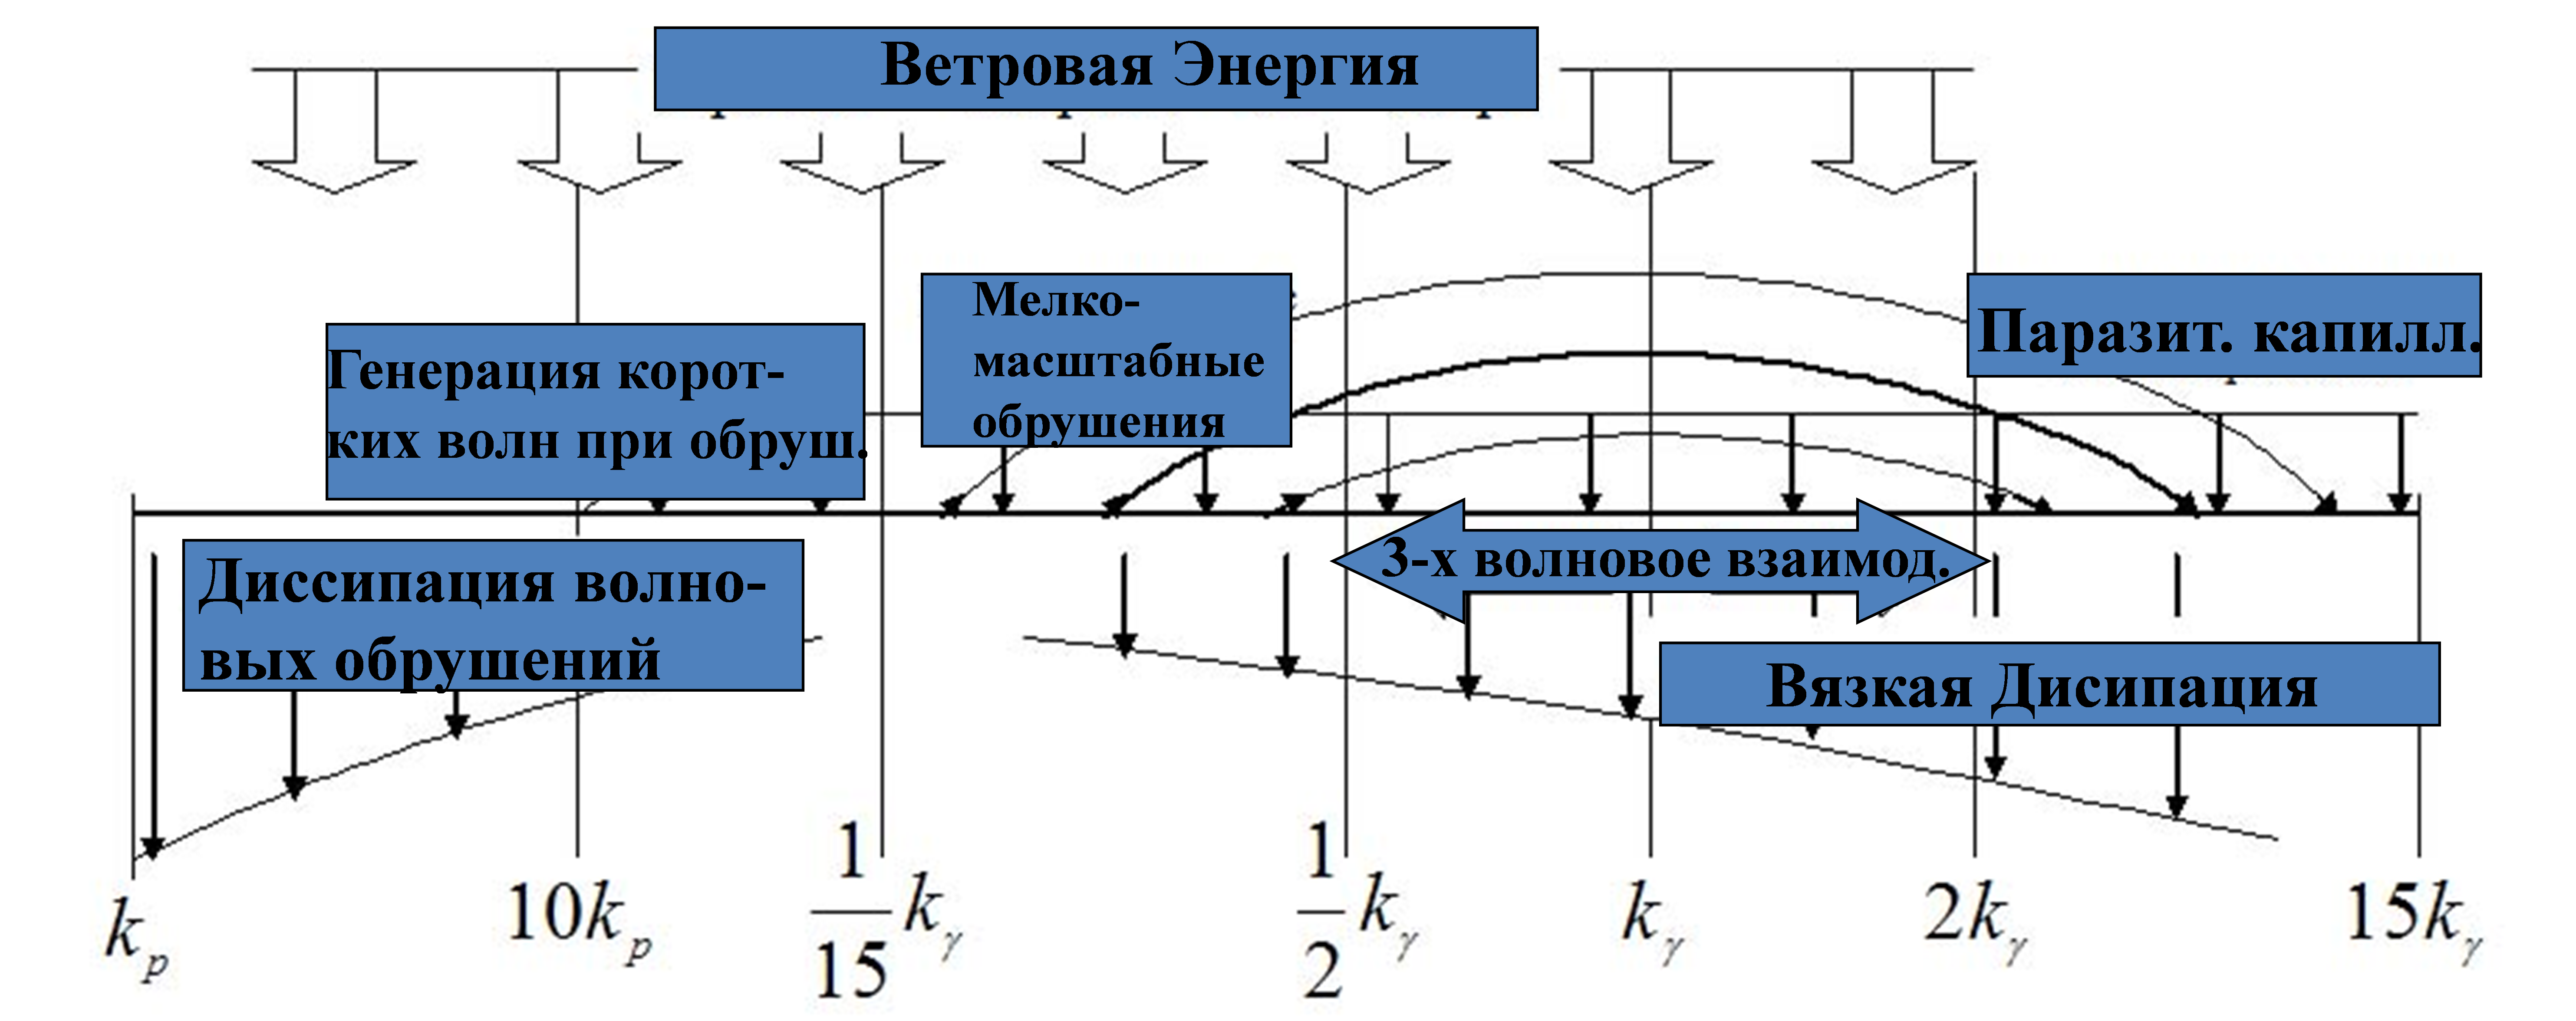
\includegraphics[width=\linewidth]{A_1}
    \floattitle{Источники и стоки энергии состоят из ветровой ``накачки», эффектов вязкой диссипации, диссипации за счёт обрушений волн, взаимодействий волн и генерации паразитных капилляров в результате обрушения волн, и могут быть представлены через уравнение}
    \caption{Источники и стоки энергии $Q(k)$}
    \label{fig:A.1}
\end{figure}


Скорость диссипации энергии в результате обрушений волн $D(k)$ в  \citep{Phillips1985} представляется в виде:



\begin{equation} \label{1.33)} D(k)=bg^{-1} c^{5} \Lambda (k), \end{equation} 



\noindent где $b$ -- эмпирическая константа порядка 0.01, а $\Lambda (k)$ -- статистическая мера обрушений волн, введённая Филлипсом \citep{Phillips1985}, таким образом, что $\Lambda (k)dk$ -- общая длина на единицу площади обрушающегося фронта поверхностных волн в диапазоне волновых чисел от $k$ to $k+dk$.

Член $Q^{nl} (k)$ в  характеризует источники и стоки энергии в результате резонансного четырёх-волнового (в гравитационном масштабе) и трёх-волнового (в капиллярно-гравитационном диапазоне) взаимодействия.

Член $Q^{wb} (k)=Q_{pc}^{wb} (k)+Q_{sw}^{wb} (k)$ описывает генерацию коротких поверхностных волн в результате обрушения волн (см. Рисунок~). В зависимости от масштаба обрушающейся волны, определяются два механизма. В первом, в результате действия поверхностного натяжения, короткие обрушающиеся волны с $k>k_{wb} $ (где $k_{wb} \approx 2\pi /0.3$рад/м) не обрушаются, а генерируют группы паразитных капилляров. Таким образом, скорость генерации паразитных капилляров (описываемых членом $Q_{pc}^{wb} (k)$) пропорциональна диссипации энергии при переносе коротких гравитационных волн с волновыми числами $k_{g} =k_{\gamma }^{2} /k$, где $k_{\gamma } =(g/\gamma )^{1/2} $ -- волновое число минимума фазовой скорости. Описание этого механизма приводится в \citep{1999a,Kudryavtsev2003}, а выражение для $Q_{pc}^{wb} (k)$ приводится ниже:



\begin{equation} \label{1.34)} \begin{array}{l} {Q_{pc}^{wb} (k)\equiv \omega ^{3} k^{-5} I_{pc} (k)} \\ {I_{pc} (k)=bk_{g}^{-1} \Lambda (k_{g} )\phi (k/k_{\gamma } ),} \end{array} \end{equation} 



\noindent где $\phi (k/k_{\gamma } )$ -- фильтрующая функция, ограничивающая действие источника $I_{pc} (k)$ в пространстве волновых чисел $k$.

При действии второго механизма, гребни более длинных обрушающихся волн с волновыми числами $k<k_{wb} $, которые обрушаются и вызывают механические возмущения морской поверхности. Этот механизм описан в статье \citep{Kudryavtsev2004}. Скорость генерации коротких волн $Q_{sw}^{wb} (k)$ изотропна и описывается через характеристики обрушений длинных волн как \citep{Kudryavtsev2004}:



\begin{equation} \label{1.35)} \begin{array}{l} {Q_{sw}^{wb} (k)\equiv \omega ^{3} k^{-5} I_{sw} (k)} \\ {I_{sw} (k)=c_{b} \omega ^{-1} \int _{0}^{k_{m} }\omega k^{-1} \Lambda (k')dk' ,} \end{array} \end{equation} 



\noindent где $c_{b} =1.2\cdot 10^{-2} $ -- эмпирическая константа; $k_{m} =\min (k/a_{b} ,k_{wb} )$ при $a_{b} =10$ -- верхний предел интегрирования, определяющий интервал обрушивающихся волн, генерирующих более короткие волны при волновом числе $k$. 



\begin{figure}[H]
    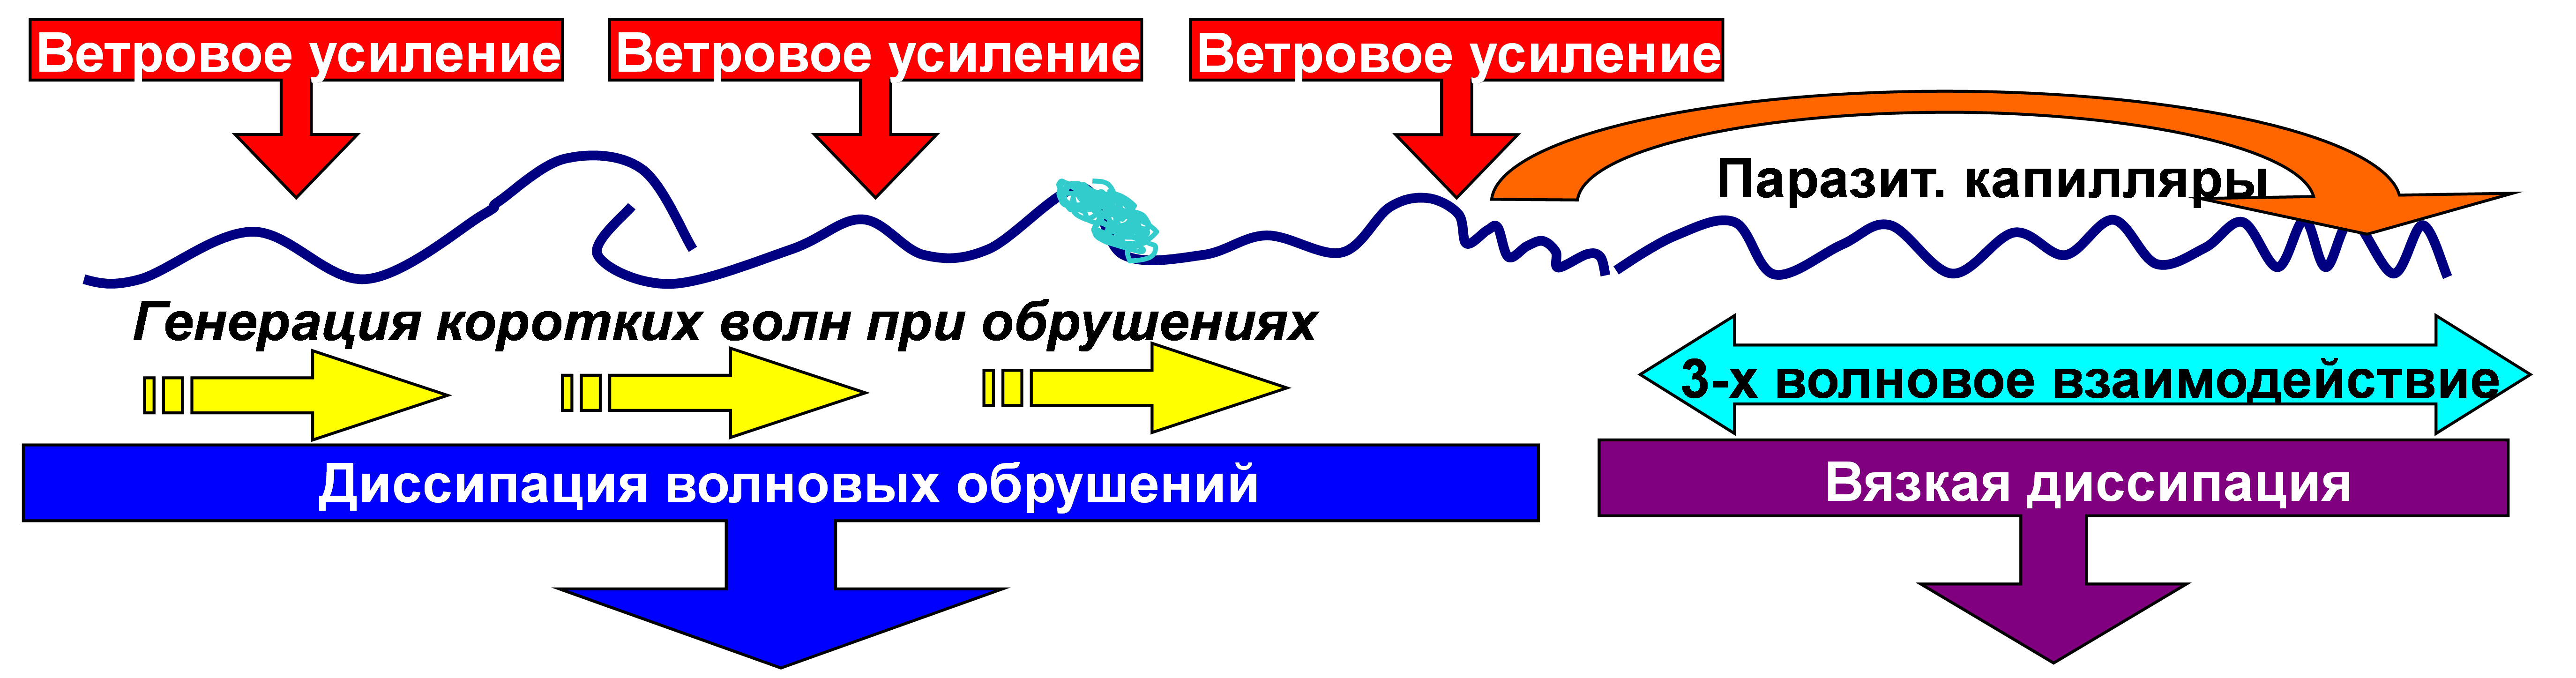
\includegraphics[width=\linewidth]{A_2}
    \floattitle{Создание ``регулярных» серий паразитных капилляров в результате действия поверхностного натяжения, при обрушении коротких волн с $k>k_{wb} $ и, вызванная обрушением гребней более длинных волн, с волновыми числами $k<k_{wb} $, механическая пертурбация морской поверхности}
    \caption{Генерация коротких поверхностных волн в результате обрушения волн}
    \label{fig:A.2}
\end{figure}


\section{Приближённое решение задачи о трансформации волн} \label{AppendixA1}

Предположим, что поля поверхностного течения и скорости ветра можно представить в пространстве Фурье:



\begin{equation} \label{1.36)} z\left(x,t\right)=\int \widehat{z}\left(K\right) \exp \left(i\left(K\cdot x-\Omega t\right)\right)dK,  \end{equation} 



\noindent где $z\left(x,t\right)$ -- произвольная константа, $\widehat{z}\left(K\right)$ -- её Фурье амплитуда (комплексная переменная), а $K$ и $\Omega $ -- вектор волнового числа и частота, соответственно. Тогда линеаризованное решение уравнения баланса действия \eqref{ZEqnNum858310} с разложением на Фурье гармоники для малых вариаций спектра, вызванных поверхностным течением и приповерхностным ветром, выглядит следующим образом \citep{Kudryavtsev2005}:



\begin{equation} \label{1.37)} T\left(k,K\right)=\frac{\tau }{1+i\cdot r} \left[\omega ^{-1} m_{k}^{ij} \widehat{u}_{ij} +\widehat{\beta }+{\left(\widehat{I}_{sw} +\widehat{I}_{pc} \right)\mathord{\left/ {\vphantom {\left(\widehat{I}_{sw} +\widehat{I}_{pc} \right) B}} \right. \kern-\nulldelimiterspace} B} \right],  \end{equation} 



\noindent где $T\left(k,K\right)={\widehat{N}\left(k\right)\mathord{\left/ {\vphantom {\widehat{N}\left(k\right) N_{0} \left(k\right)}} \right. \kern-\nulldelimiterspace} N_{0} \left(k\right)} $ -- передаточная функция, $N_{0} \left(k\right)$ -- фоновый спектр морской поверхности, определяемый локальными свойствами среды, $B$ -- спектр волн в данной точке пространства, $r$ -- безразмерный релаксационный параметр:



\begin{equation} \label{1.38)} r=\tau \omega ^{-1} \left(c_{gj} K_{j} -\Omega \right),  \end{equation} 



$m_{k}^{ij} =k_{j} {\partial \left(\ln N_{0} \right)\mathord{\left/ {\vphantom {\partial \left(\ln N_{0} \right) \partial k_{i} }} \right. \kern-\nulldelimiterspace} \partial k_{i} } $ -- тензор нормированного градиента спектра по волновым числам, $\widehat{u}_{ij} $ -- Фурье амплитуда тензора градиента скорости течения ${\partial u_{i} \mathord{\left/ {\vphantom {\partial u_{i}  \partial x_{j} }} \right. \kern-\nulldelimiterspace} \partial x_{j} } $. Оператор $m_{k}^{ij} \widehat{u}_{ij} $ в \eqref{ZEqnNum567066} можно представить в виде:



\begin{equation} \label{1.39)} \begin{array}{l} {m_{k}^{ij} \widehat{u}_{ij} =m_{k} \left(\cos ^{2} \phi \cdot \widehat{u}_{ij} -\cos 2\phi \cdot \widehat{u}_{2,2} \right)+} \\ {\qquad \, \, \, \, {1\mathord{\left/ {\vphantom {1 2}} \right. \kern-\nulldelimiterspace} 2} m_{\phi } \sin 2\phi \cdot \left(\widehat{u}_{2,2} -\widehat{u}_{1,1} \right)+} \\ {\qquad \, \, \, \, {1\mathord{\left/ {\vphantom {1 2}} \right. \kern-\nulldelimiterspace} 2} m_{k} \sin 2\phi \cdot \left(\widehat{u}_{2,1} -\widehat{u}_{1,2} \right)-} \\ {\qquad \, \, \, \, m_{\phi } \left(\sin ^{2} \phi \cdot \widehat{u}_{2,1} -\cos ^{2} \phi \cdot \widehat{u}_{1,2} \right)} \end{array},  \end{equation} 



\noindent где $m_{k} ={\partial \left(\ln N\right)\mathord{\left/ {\vphantom {\partial \left(\ln N\right) \partial \left(\ln k\right)}} \right. \kern-\nulldelimiterspace} \partial \left(\ln k\right)} $, $m_{\phi } ={\partial \left(\ln N\right)\mathord{\left/ {\vphantom {\partial \left(\ln N\right) \partial \phi }} \right. \kern-\nulldelimiterspace} \partial \phi } $, $\phi $ -- направление вектора волнового числа.

Члены $\widehat{I}_{sw} $ и $\widehat{I}_{pc} $ в \eqref{ZEqnNum567066} описывают эффект модуляции обрушений волн на коротких ветровых волнах и паразитных капиллярах.

Второй член в уравнении \eqref{ZEqnNum567066} описывает эффект влияния изменения скорости ветра на спектр волн. В частности, вариации скорости ветра могут возникать в результате трансформации атмосферного погранслоя над изменяющимся температурным фронтом в море. Также стоит отметить, что уравнение \eqref{ZEqnNum567066} описывает и модуляцию коротких волн более длинными поверхностными волнами, как например описывается в \citep{Kudryavtsev2003}.

Уравнение \eqref{ZEqnNum567066} представляет собой интегральное уравнение Фредгольма второго рода. Такое уравнение решаемо численными методами, итерационно. Тем не менее, сначала рассмотрим некоторые граничные случаи (для стационарных течений, $\Omega =0$), иллюстрирующие некоторые характеристические свойства полного решения.

В случае если параметр $r$ велик, поверхностные изменения пространственного масштаба малы, по сравнению с релаксационным масштабом $l_{r} $. Это наиболее вероятно для длинных гравитационных волн. Для $r\gg 1$ \eqref{ZEqnNum567066} сокращается до:



\begin{equation} \label{1.40)} T\left(k,K\right)=\frac{m_{k}^{ij} K_{j} \widehat{u}_{i} }{c_{gj} K_{j} } \propto -\frac{7}{2} \frac{V}{c_{g} } ,  \end{equation} 



\noindent где $V$ -- величина поверхностного течения. Это уравнение представляет трансформацию, когда поверхностные волны взаимодействуют с течением, как свободные волны и не чувствуют влияния ветра или других источников энергии. В таком случае, чем длиннее (и быстрее распространяются) поверхностные волны, тем меньше влияние поверхностного течения. Можно показать, что второй и третий член в уравнении \eqref{ZEqnNum567066} имеет порядок $r^{-1} {\widehat{u_{*} }\mathord{\left/ {\vphantom {\widehat{u_{*} } u_{*} }} \right. \kern-\nulldelimiterspace} u_{*} } $ и $r^{-1} {V\mathord{\left/ {\vphantom {V c_{g} }} \right. \kern-\nulldelimiterspace} c_{g} } $, соответственно, и их можно опустить при $r\gg 1$.

Условие, когда $r\ll 1$, выполняется для коротких ветровых волн. Здесь влияние течения пренебрежимо мало (первый член в \eqref{ZEqnNum567066} можно опустить). Вариации спектра возникают в результате локального влияния ветра и обрушений волн. Когда источником вариаций коротких волн является только ветер, \eqref{ZEqnNum567066} сокращается до:

\begin{equation} \label{1.41)} T\left(k,K\right)\approx m_{*} \frac{\widehat{u_{*} }}{u_{*} } ,  \end{equation} 



\noindent где $m_{*} $ -- спектральный показатель ветра. Таким образом, вариации в волновом спектре отражают пространственную неоднородность напряжений приводного ветра. Если же ветер однороден, единственным источником модуляции коротких волн становятся обрушения бомльших волн. Выдвигая предположение, что передаточная функция для обрушающихся волн имеет вид $T\approx m_{k}^{ij} \widehat{u}_{ij} \omega ^{-1} \tau $, модуляционная передаточная функция коротких волн может быть записана как:



\begin{equation} \label{1.42)} T\left(k\right)\approx m_{k} \frac{n_{g} +1}{n_{g} } \ln \left[\frac{k}{a_{b} k_{p} } \right]\tau \omega ^{-1} \widehat{u}_{ij} ,  \end{equation} 



\noindent где $a_{b} =10$. Чтобы вывести это уравнение, учитывался лишь первый член оператора в уравнении \eqref{ZEqnNum735720}, дающий вклад в интеграл по $\phi $. В уравнении \eqref{ZEqnNum538621} есть две отличительные особенности. Во первых -- только дивергенция поверхностного течения влияет на модуляцию коротких ветровых волн. А во вторых -- модуляция сильнее при боковом ветре, поскольку $\tau $ имеет угловую зависимость (подробнее см. \citep{Kudryavtsev2005}). Последнее утверждение предполагает, что эффект поверхностного течения приводит к анизотропии коротких ветровых волн. Проведя модельные расчёты контрастов спектра брэгговских волновых чисел для разных направлений ветра (Рисунок~34), отчётливо видно, что для бокового ветра вариации контрастов значительно выше, а для направлений против и по ветру -- они минимальны. 

В \eqref{ZEqnNum567066} заведомо не был включён член, описывающий влияние поверхностных плёнок, которые могут значительно изменять коэффициент вязкой диссипации, и, таким образом, влияют на спектр волн (см., например, \citep{Ermakov1992}). Этот механизм локализован в пространстве волновых чисел и в основном влияет на самые короткие ветровые волны, чья скорость релаксации очень велика. Поэтому можно предположить, что плёнки влияют на коротки волны локализовано в физическом пространстве и их вклад возможно учесть через изменённый коэффициент вязкости в фоновом спектре $N_{0} \left(k\right)$. Таким образом, вариации спектра насыщения волн в физическом пространстве принимают следующий вид:



\begin{equation} \label{1.43)} B\left(k\right)=B_{0} \left(k\right)\left[1+\int T(k,K)e^{i\left(K\cdot x-\Omega t\right)} dK \right],  \end{equation} 



\noindent где эффект влияния ветра и течения включены в $T(k,K)$, а поверхностных плёнок -- в $B_{0} \left(k\right)$.



\section{Трансформация СКН и обрушений волн} \label{AppendixA2}

Для создания полной модели, необходимо количественно оценить спектр волн, а также его трансформации в присутствии пространственно-неоднородных течений, переменного ветра и поверхностно-активных веществ (ПАВ), которые приводят к проявлению особенностей поверхностных течений на радиолокационных (РЛ) изображениях. Используя спектральную передаточную функцию \eqref{ZEqnNum567066}, получим вариации компонентов СКН $\Delta s_{^{j} }^{2} $ в неоднородной среде \citep{Kudryavtsev2005}:



\begin{equation} \label{1.44)} \begin{array}{l} {s_{^{j} }^{2} =s_{^{j0} }^{2} \left(1+{\Delta s_{^{j} }^{2} \mathord{\left/ {\vphantom {\Delta s_{^{j} }^{2}  s_{^{j0} }^{2} \, }} \right. \kern-\nulldelimiterspace} s_{^{j0} }^{2} \, } \right),} \\ {\Delta s_{^{j} }^{2} =\int T_{j}^{s} \left(K\right)e^{i\left(K\cdot x-\Omega t\right)}  dK,} \\ {T_{j}^{s} \left(K\right)=\iint \nolimits _{k<k_{d} }T\left(k,K\right)\kappa _{j}^{2} B\left(k\right) d\phi d\left(\ln k\right),} \end{array} \end{equation} 



\noindent где нижний индекс ``0'' означает, что СКН относится к фоновому спектру $B_{0} \left(k\right)$ в \eqref{ZEqnNum419022}, $\kappa _{j}^{2} ={k_{j} \mathord{\left/ {\vphantom {k_{j}  k}} \right. \kern-\nulldelimiterspace} k} $ -- единичный вектор волнового числа, а индекс $j=1,2$.

Область моря, покрытая обрушениями рассчитывается исходя из:



\begin{equation} \label{1.45)} \begin{array}{l} {q=q_{0} \left(1+{\Delta q\mathord{\left/ {\vphantom {\Delta q q_{0} \, }} \right. \kern-\nulldelimiterspace} q_{0} \, } \right),} \\ {\Delta q=\int T^{q} \left(K\right)e^{i\left(K\cdot x-\Omega t\right)}  dK,} \\ {T^{q} \left(K\right)=\left(n_{g} +1\right)\iint \nolimits _{k<k_{d} }T\left(k,K\right)\beta B\left(k\right) d\phi d\left(\ln k\right),} \end{array} \end{equation}



\noindent где верхний предел интегрирования относится к РЛ волновому числу как $k_{wb}^{R} =\min \left(k_{wb} ,0.1k_{r} \right)$.

На Рисунке~\ref{fig:A.3} представлена модель, отражающая механизмы, влияющие на обратное рассеяние радиолокационного сигнала, и формирование радиолокационных изображений.



\begin{figure}[H]
    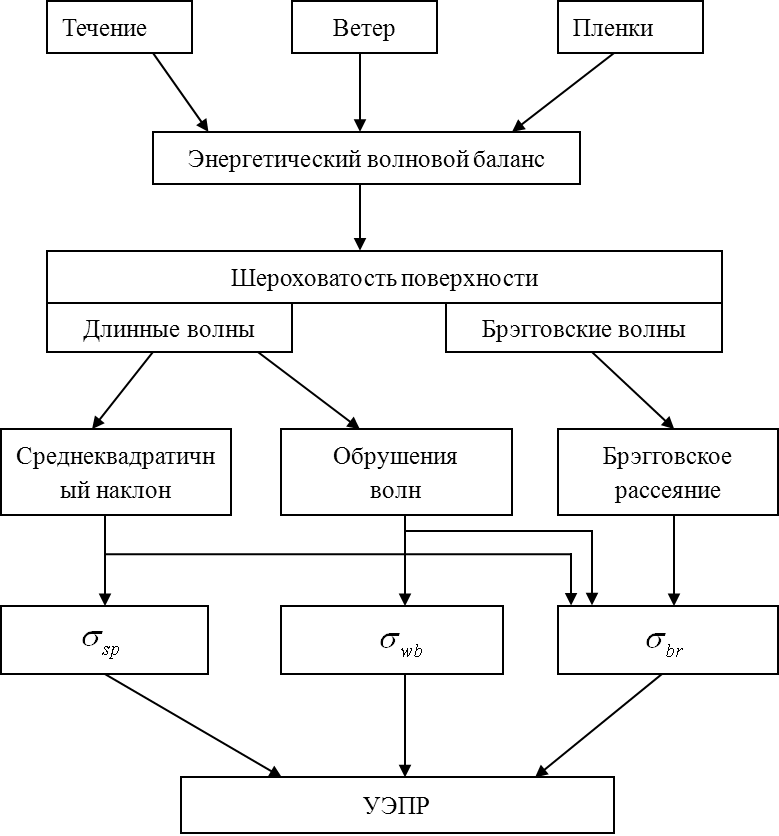
\includegraphics[width=\linewidth]{A_3}
    \floattitle{Структура механизмов модели, дающих вклад в образование радиолокационного изображения}
    \caption{Схема формирования РЛ-изображения}
    \label{fig:A.3}
\end{figure}


Примеры результата расчётов СКН и обрушений волн с использованием уравнений \eqref{ZEqnNum135284} и \eqref{ZEqnNum272976} по модели RIM приводятся на Рисунке~35.


